
\chapter{Introduction}
\label{cha:introduction}

\texttt{PAFFS} stands for "Protective Avionics Flash FS" and aims to use a minimum RAM footprint with the ability to manage multiple flashes. Most of the design ideas are inspired by the file system \texttt{JFFS3} \referenceDocument{JFFS3}, which was later extended \referenceDocument{JFFS3ex} and discontinued as predecessor of \texttt{UBIFS}.\\
The main differences to usual disk file systems are \texttt{out-of-place-writing}, a higher bit error rate and high deletion costs in terms of durability and speed. Keeping track of the files data chunks has to be different than just maintaining a big table on a disk, because the high frequented lookup table would be worn out earlier while other parts of flash will be nearly untouched. The standard approach of flash aware file systems (such as \texttt{YAFFS}) is to maintain a table-like structure in RAM and committing every chunk of new data to flash with an unique, increasing number, just like a list. This adds far more complexity to the file system as it has to scan the whole flash when mounting, but increases lifetime of the flash enormously. However, this RAM table grows linear with flash size, and thus does not scale for modern (> 2GB) flash chips. To solve this, the information has to be on flash. B+-Tree -> Section \ref{b+tree}.
Another big challenge is to reduce wear. Every change to data has to be written to another place and the old location has to be invalidated somehow. This is because the smallest unit of deletion is bigger (usually around 512 - 4086 times) than the smallest unit of a write operation. The common approach is to give every logical chunk an increasing version number. Because of the disadvantages pointed out earlier, this is not applied in \texttt{PAFFS}. Areas and address mapping -> Section \ref{areas}

\section{Fundamental structures}
\label{sec:funst}


\subsection{Areas}
\label{areas}
\paragraph{Overview}
To separate between different Types of Data. Is the logical combination of two or more erase blocks.
\begin{itemize}
	\item \texttt{AreaType} can be one of Superblock, Index, Data, (Journal). See table \ref{tab:areatypes}.
	\item Address split in \texttt{logical area n°} and \texttt{page n°}, to give way for a simple garbage collector (see  fig. \ref{fig:area_address})
	\item \texttt{AreaMap} held in flash (but cached in RAM) translates between \texttt{logical area n°} and \texttt{physical area n°}
	\item \texttt{AreaMap} also keeps record of corresponding types and usage statistics for garbage collection
	\item\texttt{AreaStatus} can be one of \texttt{closed}, \texttt{active} and \texttt{empty}. 
\end{itemize}

\paragraph{Area types}
\begin{table}[htbp]
\caption{Area types}
\label{tab:areatypes}
\begin{tabularx}{\textwidth}{lp{11cm}p{2.5cm}}
\toprule
Type & Description\\
\midrule
Superblock & One superblock area is automatically on the first area of flash, the rest is dynamically allocated. It contains the anchor blocks as well as jump pads and a superpage. See chapter \ref{sub:chainedSB} \\
Index & The index areas will contain only tree nodes (storing inodes). See chapter \ref{b+tree}.\\
Data & Data areas contain data chunks of files, directories and softlinks referenced by the index.\\
Journal & The single journal area (some when) will contain uncommitted changes to the index.\\
\bottomrule
\end{tabularx}
\end{table} 

\paragraph{Area map / Addresses}
Due to the nature of flash, any deletion is delayed as long as possible. But when free space runs low, a garbage collector has to delete dirty pages while keeping addresses valid. This is why addresses consist of two parts; a logical area number, and page offset inside this area. To read chunk of data at an address, the logical area number has to be translated to a physical area via the \texttt{AreaMap}. It is stored in the superpage (see chapter \ref{sub:chainedSB}), but is cached in RAM.\\
This area map grows linear in size with area count which is by itself depended by block count divided by area size.\\
The size of an area is a trade-off between low RAM usage (big areas) and a more efficient garbage collection (small areas). In this test environment, an area size of two erase blocks is chosen\footnote{Which should be the minimum size, because the anchor area has to be two blocks in size.}. With a normal 2GB flash chip\footnote{2048 Byte user data per page, 1024 pages per block, $\approx 2^21$ blocks.}, this configuration would use $(3+2+16+32+32) / 8 * 2^{21} / 2 = 11141120$ Byte $= 10,625$ MB RAM. Increasing the size of an area to 8 erase blocks would result in 2,65 MB usage, which would suit the requirements better.

\paragraph{Area summary}
To distinguish between \texttt{free}, \texttt{used} and \texttt{dirty} pages, a per-area list is held in area summary cache. The Information is used by the garbage collection copying only used pages to a new area, by the function looking for free pages for writing data or index chunks, and by runtime sanity checks. The Caching techniques are described in chapter \ref{ascache}.

\subsection{Garbage collection}
\paragraph{Functionality}
The garbage collection needs at least one free area to copy valid data to. At first, one or more of the \texttt{closed} areas are inspected (as the \texttt{active} areas are still in use), sorted by textt{dirty} pages and eventually chosen for garbage collection. All valid pages are copied from the old area to the new area in their same relative positions. After that, the old area is erased, and the \texttt{AreaMap} is updated so that the logical areas swap their physical positions. The new area is marked \textit{active}, and the \texttt{AreaSummary} is deleted from Flash, thus giving way for a new commit of an area summary. If the previous way is not sufficient, the \texttt{garbage buffer} is given up for storing the last information. This procedure can not be reverted, and is reserved for \texttt{index} type only to enable a safe unmount without information loss.
\begin{figure}[ht]
  \centering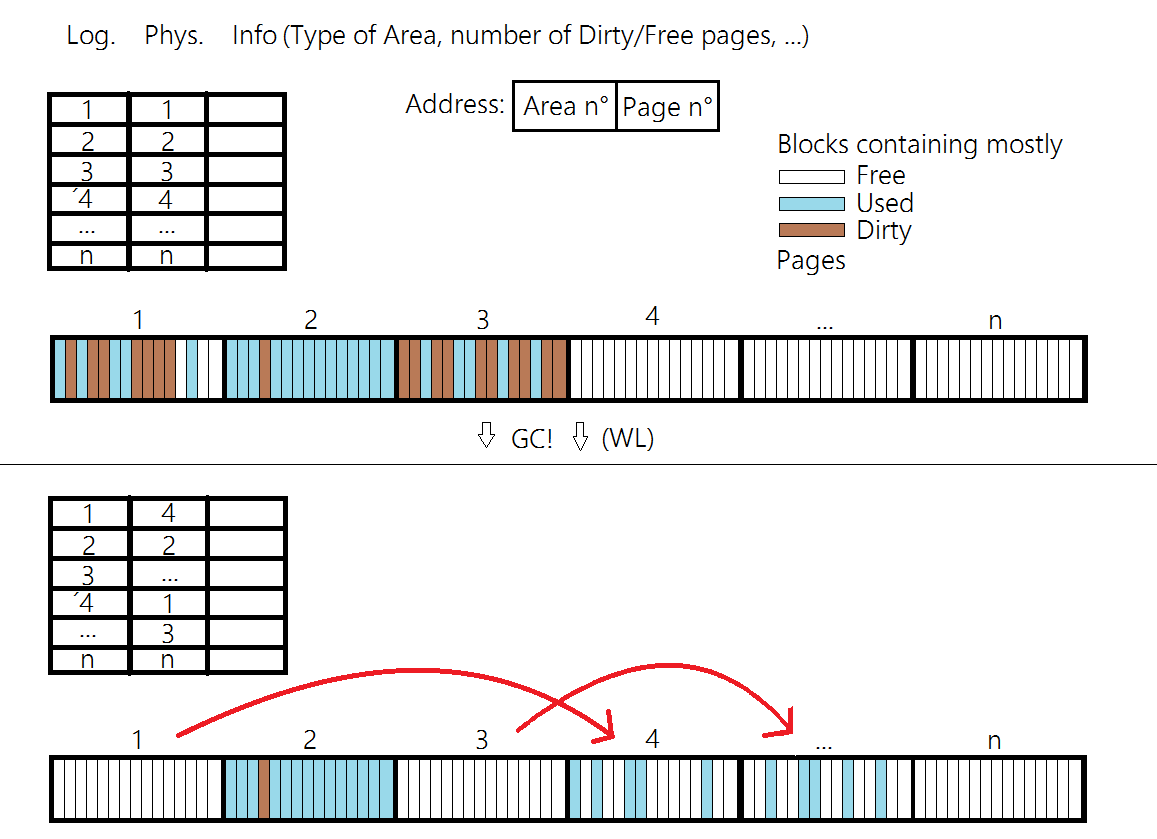
\includegraphics[width=\textwidth]{Areas_address.png}
  \caption{Basic process of garbage collection with areas}
  \label{fig:area_address}
\end{figure}

\subsection{Area Summary Cache}
\label{ascache}
Yes.

\subsection{Chained superblock}
\label{sub:chainedSB}
\paragraph{Overview}
Along with some static information, keeping an index requires having some sort of start point to find the first address of a table or the first position of a root node. The naive approach is having the first block contain this dynamic information. However this is bad practice, as it wears off the first (or first $n$) blocks enormously while leaving other places barely used. Another approach is to scan the whole flash for something with an unique sequential number, which is unacceptable as mount time scales linear with flash size.
The following structure of a chained superblock provides wear levelling of the first blocks and enables logarithmic mount time.
For a more detailed explanation see \referenceDocument{JFFS3} Chapter 4.

\paragraph{Functionality}
The first area of a flash contains two consecutive anchor blocks. The one page with the highest (i.e newest) number inside the anchor blocks is considered valid. This anchor page holds static information like file system version, number of blocks and the like as well as the address to the first jump pad located somewhere in a superblock area. these jump pads reference either a next pad or the superpage which is a page within a superblock area. This page holds frequently changed values like the address to the root node of the index tree and the area map.\\

When a change of the index tree has been committed to flash, the new address of the root node has to be written to a new superpage. The address of the new superpage is then appended to the last jump pad block. If this block is full, it will be erased and the new address is written to a new jump pad block. This requires the next higher-level jump pad to append the address of the new jump pad block, and so on. When one of the anchor blocks is full, first the anchor page is written to the other block, and then the first block is deleted.\\



\subsection{Tree Indexing}
\label{b+tree}
\paragraph{Overview}
B+Tree is a variation of the standard binary search tree with more than two keys per node and having all actual data only in leaves. This increases space for keys and therefore the fanout. Variable size, minimum tree height + 1\footnote{Check if true.}. Tree height is $log(n)$, and so is search, insert and delete $\mathcal{O}log(n)$. Because of \textit{out-of-place-write}, with every change to a single inode, the whole path up to the root node has to be updated (see figure \ref{fig:btreewandering}). To heavily decrease flash wear, a caching strategy is used. Any modification to the tree is held back in RAM as long as possible, until cache memory is running low. During cache flush all dirty nodes are committed to flash and freed in main memory. This caching can save 98\% of flash operations and speed up access times as well (see \referenceDocument{b+Tree}). Depending on cache flush strategy, all branch nodes are kept in cache while leaves are removed. This increases cache-hit ratio because there are less branches than leaves, but they branches more likely to be accessed again.

\begin{figure}[htp]
	\centering
	\begin{subfigure}[t]{.9\textwidth}
		\centering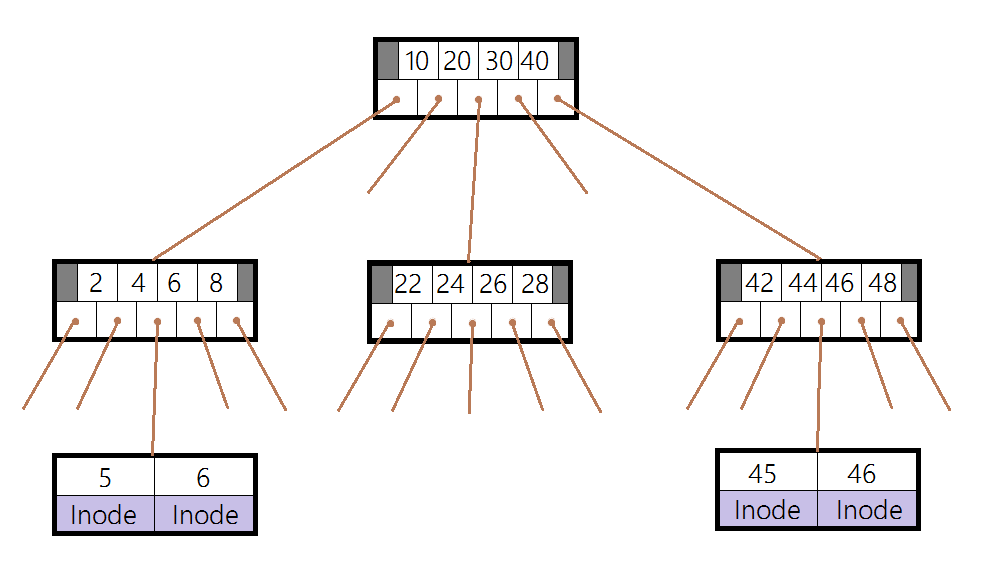
\includegraphics[width=\textwidth]{btree.png}
		\subcaption{Before}
	\end{subfigure}\\
	\begin{subfigure}[t]{.9\textwidth}
		\centering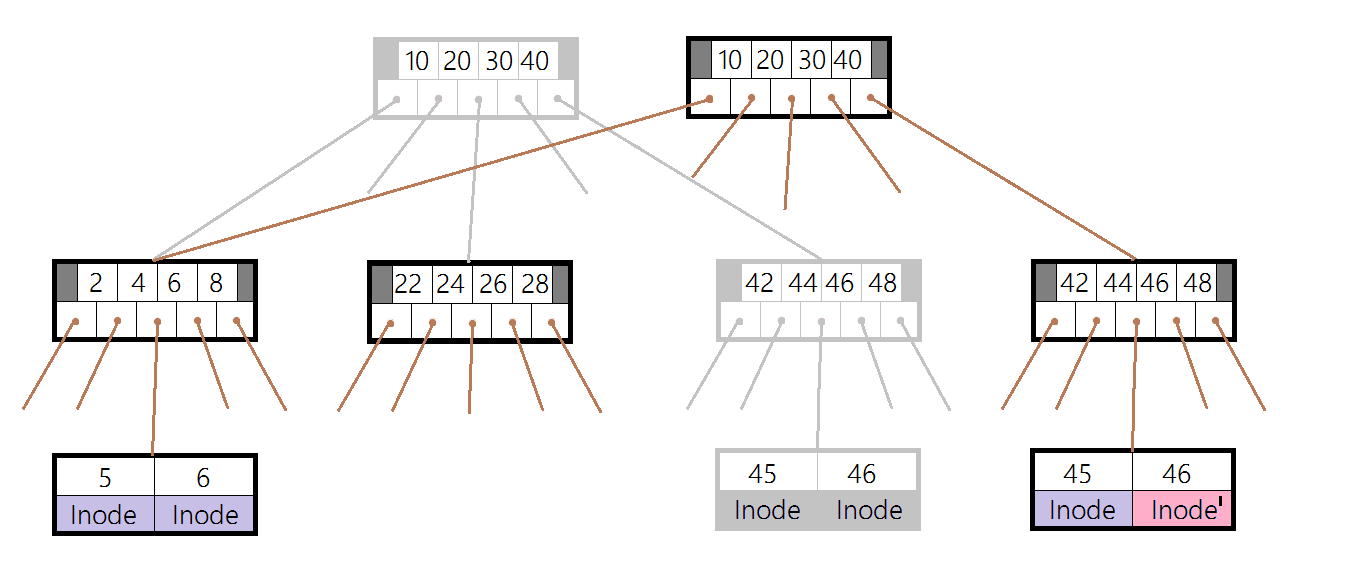
\includegraphics[width=\textwidth]{btree_2.png}
		\subcaption{After}
	\end{subfigure}
	\caption{\label{fig:btreewandering}B+-Tree after updating a single inode. The whole path has to be rewritten.}
\end{figure}

\begin{figure}[htp]
	\centering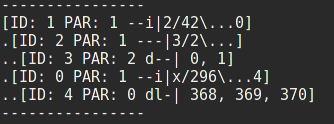
\includegraphics[width=\textwidth]{TreeCachePrint.PNG}
	\caption{\label{fig:TreeCachePrint}Example output of a cache content visualization. Notice the \texttt{dirty}, \texttt{locked} and \texttt{inherited lock} flags.}
\end{figure}

\subsection{Inodes}
\label{inode}
\paragraph{Overview}
Can be file, directory and softlink. Points to data chunks in a way like \texttt{EXT3} does. See Table \ref{tab:pinode}. It is possible to use pointer space for very small files or directories (14 * 4 Byte).
\begin{table}[htbp]
\caption{Inode contents}
\label{tab:pinode}
\begin{tabularx}{\textwidth}{lp{11cm}p{2.5cm}}
\toprule
Value & Description\\
\midrule
\texttt{pInode\_no} & Unique number of inode. \\
\texttt{pInode\_type} & One of \texttt{file}, \texttt{directory} or \texttt{link}.\\
\texttt{permission} & Global read, write and execute permissions. Changeable via \texttt{chmod}.\\
\texttt{created} & Unix time stamp of file creation.\\
\texttt{modified} & Unix time stamp of last file write access.\\
\texttt{size} & Size of user data in bytes. \\
\texttt{reserved size} & Space user data is actually occupying in bytes (multiple of chunk size).\\
\texttt{direct pointer} & 11 direct pointers to user data chunks.\\
\texttt{indirect pointers} & One of each first, second and third layer indirection pointers pointing to data chunks with more pointers.\\
\bottomrule
\end{tabularx}
\end{table} 

\section{Tests}
\begin{flushleft}
	
\end{flushleft}
This section is under development since the filesystem is unfinished. Meanwhile look at fancy pictures:

\begin{figure}[htp]
	\centering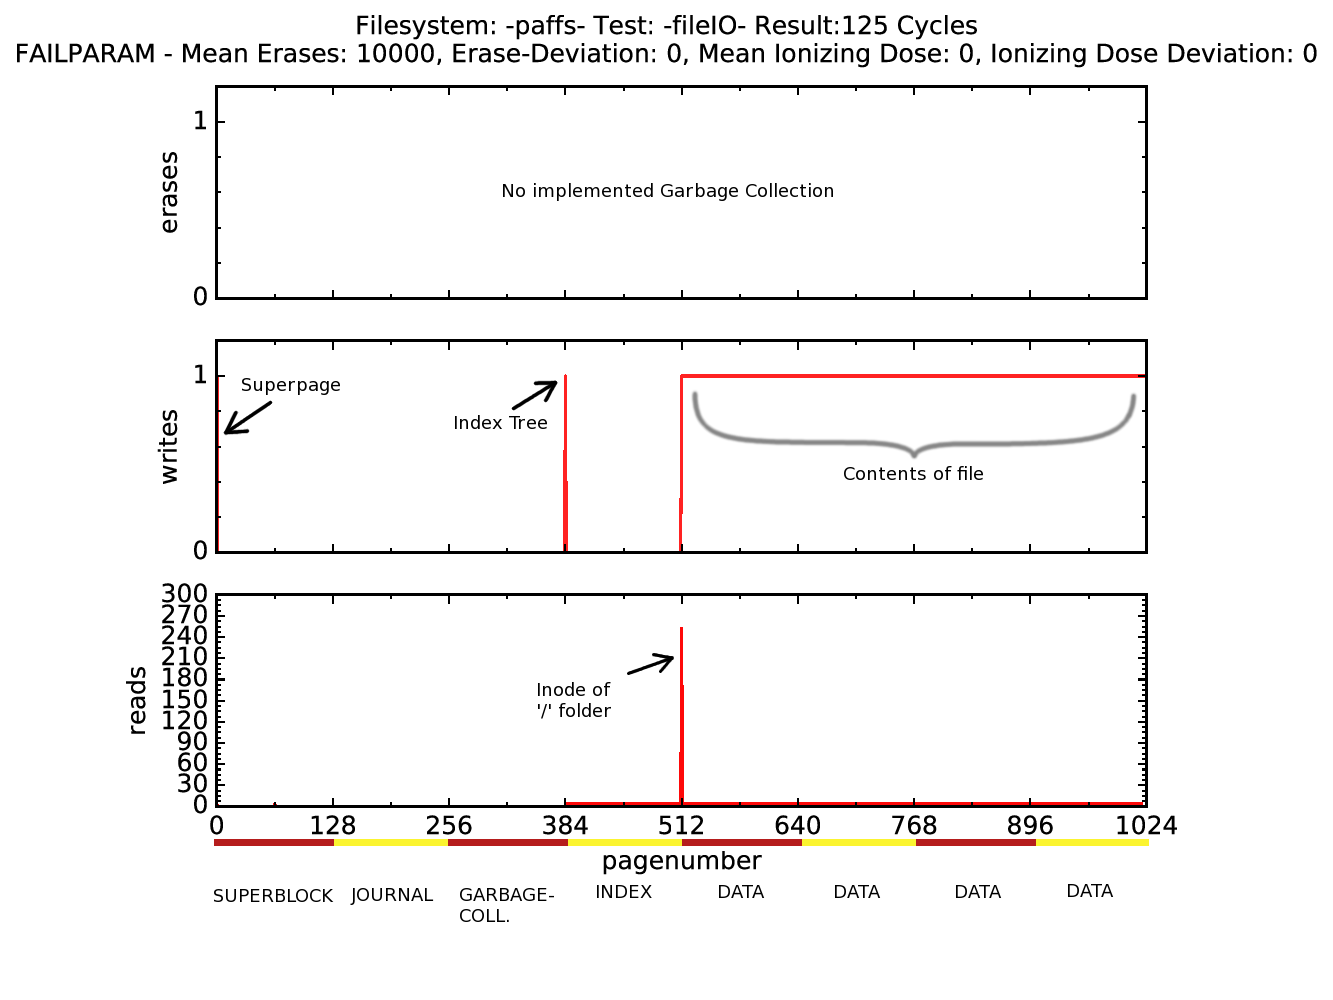
\includegraphics[width=\textwidth]{paffs__fileIO_annotations.png}
	\caption{\label{fig:fileIO} Status of simulated flash after 125 read/write cycles on a single file.\\TODO: Change "contents of file" to "Dirty or used Pages of file"}
\end{figure}
\begin{figure}[htp]
	\centering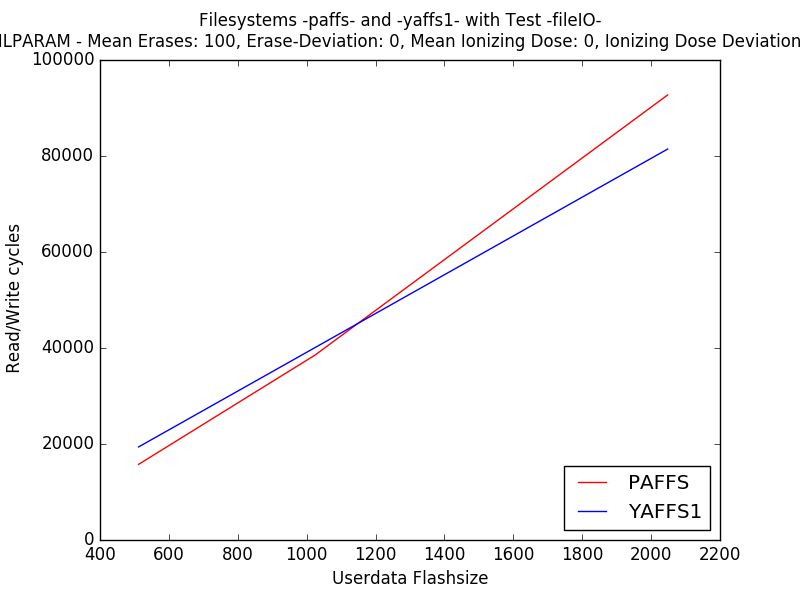
\includegraphics[width=\textwidth]{yaffs_paffs_comparison_WL.png}
	\caption{\label{fig:fileIOCompare} Comparison of wear levelling performance as a function of flash size between PAFFS and YAFFS1.}
\end{figure}


\appendix
\section{TODOS}
\begin{itemize}
	\item When ASCache runs full, some used pages cant be marked as dirty. Build sanity checker, scanning whole FS and marking unreachable pages as such.
	\item Implement dynamic count of submitted areas to superpage. (Maybe call it Checkpoint?)
	\item CRC and ECC. How will a broken FS be transferred into a safe state?
	\item Merge DATA and INDEX areas to a single DATA type. Benefits: Less complexity, more efficient space usage, GC desperate mode for unmounting only.
	\item TreeCache - full commit from time to time. (Maybe 'used' marker?)
	\item GC: Static Wear levelling, keep deletioncount in mind.
	\item Implement additional driver function for copying pages for optimizing.
	\item Replace mallocs to variable sized arrays. (Or standard container, b/c variable sized arrays are not legal in c++)
	\item Use Inode pointer space for very small files to speed up access and save space.
	\item Implement Inode and DATA Buffer to speed up everything. Note: Low priority and high effort.
\end{itemize}
